\documentclass[10pt,a4paper]{article}

\usepackage[T1]{fontenc}
\usepackage[utf8]{inputenc}
\usepackage{lmodern}
\usepackage[scaled=0.92]{helvet}
\renewcommand{\familydefault}{\sfdefault}
\renewcommand{\ttdefault}{lmtt}
\usepackage[italic]{mathastext}
\usepackage{amsmath,amssymb}
\usepackage{microtype}
\usepackage[a4paper,left=1.75cm,right=1.75cm,top=1.65cm,bottom=1.7cm,headheight=19pt]{geometry}
\usepackage{ragged2e}
\usepackage{booktabs}
\usepackage{tabularx}
\usepackage{array}
\usepackage{enumitem}
\usepackage{listings}
\usepackage[table]{xcolor}
\usepackage{tcolorbox}
\usepackage{tikz}
\usetikzlibrary{arrows.meta,positioning,fit,backgrounds,calc}
\usepackage{titlesec}
\usepackage{fancyhdr}
\usepackage[colorlinks=true,linkcolor=navy,urlcolor=teal,citecolor=teal]{hyperref}
\usepackage[font=small,labelfont=bf,textfont=small]{caption}
\renewcommand{\figurename}{Figure}
\renewcommand{\tablename}{Table}

\definecolor{navy}{HTML}{12355B}
\definecolor{teal}{HTML}{0F7B6C}
\definecolor{amber}{HTML}{B9770E}
\definecolor{crimson}{HTML}{A33A32}
\definecolor{ink}{HTML}{1F2933}
\definecolor{mist}{HTML}{F2F5F7}
\definecolor{slate}{HTML}{5B6770}

\color{ink}
\RaggedRight
\setlength{\parindent}{0pt}
\setlength{\parskip}{2.2pt}
\renewcommand{\arraystretch}{1.12}
\setlist[itemize]{leftmargin=1.05em,itemsep=1.2pt,topsep=2pt,parsep=0pt}
\setlist[enumerate]{leftmargin=1.25em,itemsep=1.2pt,topsep=2pt,parsep=0pt}

\titleformat{\section}{\large\bfseries\color{navy}}{\thesection.}{0.45em}{}
\titlespacing*{\section}{0pt}{7pt plus 2pt minus 1pt}{2pt}
\titleformat{\subsection}{\normalsize\bfseries\color{teal}}{\thesubsection}{0.45em}{}
\titlespacing*{\subsection}{0pt}{5pt plus 1pt minus 1pt}{1pt}
\titleformat{\paragraph}[runin]{\normalsize\bfseries\color{navy}}{}{0pt}{}[\hspace{0.4em}]
\titlespacing*{\paragraph}{0pt}{3pt}{0.4em}

\pagestyle{fancy}
\fancyhf{}
\fancyhead[L]{\footnotesize\bfseries\color{navy}Xplainable}
\fancyhead[R]{\footnotesize\color{slate}Technical report \textperiodcentered{} More than a Hack 2027}
\fancyfoot[C]{\footnotesize\color{slate}\thepage}
\renewcommand{\headrulewidth}{0.35pt}
\renewcommand{\headrule}{\hbox to\headwidth{\color{navy!35}\leaders\hrule height \headrulewidth\hfill}}

\lstset{
  basicstyle=\ttfamily\footnotesize,
  backgroundcolor=\color{mist},
  frame=none,
  breaklines=true,
  columns=fullflexible,
  keepspaces=true,
  showstringspaces=false,
  aboveskip=2pt,
  belowskip=2pt,
  xleftmargin=3pt,
  xrightmargin=3pt
}

\newcommand{\good}[1]{\textcolor{teal}{\bfseries #1}}
\newcommand{\bad}[1]{\textcolor{crimson}{\bfseries #1}}
\newcommand{\code}[1]{\texttt{\small #1}}
\newcommand{\sha}[1]{\texttt{\scriptsize #1}}

\hypersetup{
  pdftitle={Xplainable - Frame-by-frame possession},
  pdfauthor={Team Xplainable},
  pdfsubject={More than a Hack 2027 - Phase 1: Possession},
  pdfkeywords={HMM, possession, soccer, tracking, YOLO, spellF1}
}

\begin{document}
\thispagestyle{empty}

% ----------------------------------------------------------------------------- title
\begin{tcolorbox}[colback=white, colframe=white, boxrule=0pt, left=0pt, right=0pt, top=0pt, bottom=0pt]
{\footnotesize\bfseries\color{teal}MORE THAN A HACK 2027 \textperiodcentered{} PHASE 1: POSSESSION}\\[3pt]
{\fontsize{30}{32}\selectfont\bfseries\color{navy}Xplainable}\\[2pt]
{\Large\color{ink}Frame-by-frame possession over tactical tracking}\\[5pt]
{\small\color{slate}FC Barcelona -- Athletic Club \textperiodcentered{} 199,319 frames \textperiodcentered{} 25 fps \textperiodcentered{} 105.3 $\times$ 68.0 m \textperiodcentered{} November 17, 2026}\\[3pt]
{\small\color{slate}\textbf{Team Xplainable:} Joan Ignasi Cid \textperiodcentered{} Julian Bascones \textperiodcentered{} Mercè Tormo \textperiodcentered{} Aran Roig \textperiodcentered{} Miguel Robledo}
\end{tcolorbox}

\vspace{-2pt}
{\color{navy!30}\rule{\textwidth}{0.7pt}}
\vspace{2pt}

\begin{center}
\begin{tabular}{@{}c@{\hspace{2.1cm}}c@{\hspace{2.1cm}}c@{\hspace{2.1cm}}c@{}}
{\fontsize{19}{20}\selectfont\bfseries\color{navy}0.9257} &
{\fontsize{19}{20}\selectfont\bfseries\color{navy}0.9661} &
{\fontsize{19}{20}\selectfont\bfseries\color{navy}18 / 17} &
{\fontsize{19}{20}\selectfont\bfseries\color{navy}199,319}\\[-1pt]
{\footnotesize\color{slate}public spellF1} &
{\footnotesize\color{slate}macroF1 (H/A/D)} &
{\footnotesize\color{slate}predicted / GT possessions} &
{\footnotesize\color{slate}CSV rows}
\end{tabular}
\end{center}
\vspace{-1pt}
% ----------------------------------------------------------------------------- resumen
\section{Summary and approach}

The goal is to assign each of the 199,319 frames of the match one of four states:
\good{H} (Barcelona possession), \good{A} (Athletic Club), \good{D} (dead ball or out of
play) or \good{X} (abstention). The submission is a single CSV of 199,319 rows produced by a
deterministic chain, with no manual labels and no use of the private ground truth. The
difficulty is not guessing the average frame: it is \emph{not fragmenting possessions}. The
metric that decides the ranking, \texttt{spellF1}, matches whole possessions; a spurious one
second switch can destroy a correct thirty second one.

Our starting point is the tactical ATD: 46 anonymous slots, no player identity, and the ball
observed in only \textbf{56.9\,\%} of the frames (2.2\,\% estimated and 40.8\,\% with no
estimate at all). On that base we build three layers. First, a \textbf{three-state HMM} with
strong persistence, geometric emissions and an explicit gap model. Second, a
\textbf{perception layer} with two YOLO26x detectors (ball and players) and a \textbf{log
opinion poll} that folds in independent evidence without replacing the HMM. Third, a
\textbf{transition layer} driven by physical events --- kicks, controls and contacts --- that
turns a smooth tracking signal into correct possessions.

The reason for this design is twofold. With only five minutes of public ground truth, an
end-to-end model would learn to copy that window; an auditable HMM plus physical rules, by
contrast, can be verified, run on CPU and reproduced byte for byte. And the possession
literature agrees with the intuition: possession changes are discrete events (a kick, a
control, an interception), not a continuous drift of distances. The HMM brings stability; the
events bring the moment.

On the public window (7,500 frames, 17 possessions) the HMM with fusion scores
\textbf{0.6519} spellF1. The transition layer lifts it to \textbf{0.9257}, with macroF1
\textbf{0.9661} and accuracy \textbf{0.9689}. The 95\,\% bootstrap interval for spellF1 is
[0.857; 0.971]: with 17 possessions it is wide, and a small difference should not be read as
a real improvement.

\begin{center}
\small
\captionof{table}{Public evaluation window: frames 11,185--18,684 (7,500), 17 GT possessions
and a mean duration of 14.2 s. The right-hand column is the file submitted. The bootstrap uses
2,000 resamples.}
\label{tab:metrics}
\begin{tabular}{lrr}
\toprule
Metric & HMM + fusion & \textbf{+ transitions} \\
\midrule
spellF1 (primary) & 0.6519 & \textbf{0.9257} \\
spellF1 at IoU 0.5 & 0.6667 & 0.9143 \\
macroF1 (H/A/D) & 0.9469 & \textbf{0.9661} \\
accuracy & 0.9420 & 0.9689 \\
Cohen's kappa & 0.9087 & 0.9507 \\
class-D F1 & 0.9733 & 0.9574 \\
team accuracy (both live) & 0.9405 & 0.9815 \\
predicted possessions & 10 & 18 \\
mean possession duration & 24.0 s & 13.6 s \\
95\,\% bootstrap for spellF1 & [0.430; 0.817] & [0.857; 0.971] \\
\bottomrule
\end{tabular}
\end{center}

The transition layer lowers the class-D F1 slightly (0.9733 $\to$ 0.9574) because it converts
some \emph{dead ball} frames close to the event into the possession of the team that triggers
it. It is a deliberate trade-off: spellF1 rises 27.4 points and the macroF1 improves as well.
The rest of this note explains how each decision is taken and where it fails.

% ----------------------------------------------------------------------------- arquitectura
\section{Architecture}

Figure~\ref{fig:arch} shows the full chain. Assets enter only once; each layer produces a
verifiable intermediate artefact. Perception is the only stage that needs a GPU; fusion,
transitions, explainer and viewer are deterministic CPU.

\begin{figure}[t]
\centering
\begin{tikzpicture}[
  font=\scriptsize,
  input/.style={draw=slate!55, fill=mist, rounded corners=1.5pt, align=center, inner sep=2.4pt, minimum height=8.5mm, text width=2.8cm},
  model/.style={draw=teal!85!black, fill=teal!8, rounded corners=2pt, align=center, inner sep=3pt, minimum height=11mm, text width=5.1cm},
  wide/.style={draw=navy, fill=navy!6, rounded corners=2pt, align=center, inner sep=3pt},
  inner/.style={draw=amber!85!black, fill=amber!10, rounded corners=1.5pt, align=center, inner sep=2.2pt, text width=3.75cm, minimum height=10mm},
  output/.style={draw=navy, fill=navy!12, rounded corners=2pt, align=center, inner sep=3pt, minimum height=10mm, text width=5.5cm},
  arr/.style={-{Latex[length=1.5mm]}, draw=slate!70, line width=0.55pt},
  bus/.style={draw=slate!70, line width=0.7pt}
]
% inputs
\node[input] (atd) at (2.0,0)  {\textbf{Tactical ATD}\\ball + 46 slots};
\node[input] (tags) at (5.2,0) {\textbf{Smart tags}\\638 intervals};
\node[input] (hom) at (8.4,0)  {\textbf{Homography}\\105.3 $\times$ 68.0 m};
\node[input] (aud) at (11.6,0){\textbf{MP4 audio}\\whistle 2.4--3.8 kHz};
\node[input] (vid) at (14.8,0){\textbf{Tactical video}\\199,319 frames};
\node[font=\scriptsize\bfseries, text=navy, anchor=south west] at (0.0,0.62) {INPUT ASSETS};
% bus
\draw[bus] (0.25,-1.18) -- (16.55,-1.18);
\foreach \n in {atd,tags,hom,aud,vid} \draw[arr] (\n.south) -- ++(0,-0.28);
% models
\node[model] (hmm) at (4.5,-2.65) {\textbf{Base HMM (ATD)}\\emissions $q_H,q_A,q_D$ \textperiodcentered{} Viterbi\\persistence $p_{stay}=0.995$};
\node[model] (yolo) at (11.5,-2.65) {\textbf{YOLO26x perception}\\ball + players at 1024 px\\physical gate 40 m/s $+$ 1 m};
\draw[arr] (4.5,-1.18) -- (hmm.north);
\draw[arr] (11.5,-1.18) -- (yolo.north);
% poll
\node[wide, text width=14.5cm, minimum height=9mm] (poll) at (8.4,-4.55)
  {\textbf{Multi-source poll (8 voters):} HMM 1.00 \textperiodcentered{} YOLO ball 0.10 \textperiodcentered{} players 0.10 \textperiodcentered{} ATD 0.02/0.01 \textperiodcentered{} tags 0.01 \textperiodcentered{} audio 0.02 \textperiodcentered{} events 1.00 (hard D)};
\draw[arr] (hmm.south) -- ++(0,-0.3) -| ([xshift=-2.6cm]poll.north);
\draw[arr] (yolo.south) -- ++(0,-0.3) -| ([xshift=2.6cm]poll.north);
% transition layer
\node[wide, text width=14.5cm, minimum height=20mm] (transbg) at (8.4,-7.02) {};
\node[font=\scriptsize\bfseries, text=navy, anchor=north] at (8.4,-6.05) {TRANSITION LAYER (events $\rightarrow$ possessions)};
\node[inner] (det) at (3.35,-7.28) {\textbf{1 \textperiodcentered{} Detect}\\kicks, onsets, contacts\\and keeper hands};
\node[inner] (gate) at (8.4,-7.28) {\textbf{2 \textperiodcentered{} Filter}\\different team, live ball\\evidence $\geq 0.10$ for 2 s};
\node[inner] (rede) at (13.45,-7.28) {\textbf{3 \textperiodcentered{} Re-decode}\\logit pulse + Viterbi\\+ restart rules};
\draw[arr] (poll.south) -- (transbg.north);
% outputs
\node[output] (csv) at (4.6,-9.35) {\textbf{Xplainable.csv}\\199,319 rows \textperiodcentered{} H/A/D/X};
\node[output, draw=amber!85!black, fill=amber!8] (view) at (12.2,-9.35) {\textbf{Explainer + viewer}\\why each possession changes};
\draw[arr] (transbg.south) -- ++(0,-0.25) -| ([xshift=-1.5cm]csv.north);
\draw[arr] (transbg.south) -- ++(0,-0.25) -| ([xshift=1.5cm]view.north);
\end{tikzpicture}
\caption{Four-stage architecture. Perception and the HMM produce independent votes; the poll
weights them with the HMM as anchor; the transition layer detects events, filters them and
re-decodes. The public ground truth is only used in evaluation (it does not appear in the
figure because it is not an input).}
\label{fig:arch}
\end{figure}
\paragraph{Assets.} The ATD supplies the ball and 46 slots (24 Barcelona, 22 Athletic) in
metres, at 25 fps, with $x=0$ at the Barcelona goal. The smart tags supply 638 intervals and
14 codes (restart types, progression, chance, goal); throw-ins arrive without a team. The
homography is used to validate the geometry and to project the viewer, never as a label. The
MP4 audio feeds the whistle detector. The tactical video feeds the YOLO perception.

\paragraph{Perception.} Two YOLO26x detectors at 1024 px, trained \emph{only} on external
data, produce player and ball boxes. The feet are projected to metres with the homography;
each player's team is taken from the nearest ATD slot (no identity or shirt colour is
asserted). A physical gate of $40\ \mathrm{m/s}+1\ \mathrm{m}$ rejects unreachable
detections, and acquiring or re-acquiring a track requires two mutually reachable
detections. The own tracker anchors to the ATD while the ATD sees the ball and only accepts
video measurements inside the gate; if it has neither anchor nor measurement, it declares
itself \emph{lost}. On the public window 4,497 YOLO observations were accepted: the raw
detections had 566 jumps above 2.6 m per frame (maximum 84.9 m); after the gate, no
consecutive pair exceeds it (maximum 1.86 m).

\paragraph{Fusion.} Each source emits a probability over H/A/D. The poll is a log-opinion
mixture anchored in the HMM:
\begin{equation}
\log p \;\propto\; w_{\mathrm{hmm}}\log q_{\mathrm{hmm}}
\;+\;\sum_i w_i \log p_i,
\qquad w_{\mathrm{hmm}}=1.00 .
\label{eq:pool}
\end{equation}
The weights are a design prior, not tuned against the ground truth. ATD, tags and audio weigh
little because they are already inside the HMM emission; counting them again would duplicate
evidence. YOLO and the YOLO players are the independent evidence. Confirmed events are a hard
$D$. After the poll, a temporal HMM with the same prior decodes the sequence. Fusion by
itself does not improve the spellF1 (0.6519): it is a safety and evidence layer for the next
stage, not a substitute for the HMM.

\paragraph{Transitions.} This is the layer that brings the gain. The poll is a smoother: the
HMM concentrates about 2.7 nats of temporal evidence and the evidence votes add less than
0.5 nats, so a real one-frame change decodes late or is lost. The layer detects the physical
event, attributes it to a team, checks that the independent evidence backs it and re-decodes
with a decaying pulse on the incoming team's logit, a relaxed transition matrix around the
event and protection so that the later smoothing does not absorb the spell. Over the full
match 194 kicks and 23 onsets were detected; the gates discarded 1,004 candidates and 100
events were kept.

% ----------------------------------------------------------------------------- modelos
\section{Models}

\subsection{Base HMM: stability and gaps}

The HMM has three states and four deliberately sticky transition probabilities:
\begin{equation}
p_{stay}=0.995,\qquad p_{ha}=0.0005,\qquad p_{hd}=0.001,\qquad p_{dh}=0.007,
\label{eq:trans}
\end{equation}
The D row closes with $1-2p_{dh}=0.986$. With the ball visible, the emission compares the
ball's distance to the nearest player of each team, with $\sigma=4.0$ m:
\begin{equation}
q_H=e^{-d_H^2/(2\sigma^2)},\qquad
q_A=e^{-d_A^2/(2\sigma^2)},\qquad
q_D=\operatorname{sigmoid}\!\left(\frac{\min(d_H,d_A)-8.0}{1.5}\right)+\cdots
\label{eq:emis}
\end{equation}
The $q_D$ part adds independent dead-ball evidence: ball out of the field, ball stopped next
to a line, team movement energy and the parked-ball-on-the-touchline pattern. If the ball is
more than 7 m from all players it is considered loose or in flight and the emission is
uniform; if it is also moving at less than 2 m/s, the last team to touch it receives
70\,\% of the mass when the touch is less than 5 s old. For gaps of up to 120 frames
(4.8 s) the emission is uniform; for longer gaps the shape of the team around the last known
position and the distance to the line are used, with a weak prior. With fewer than 6 visible
players it is treated as absent evidence, not as a team.

The decode is a per-half Viterbi with 500 frames of context. The scored halves are
[11,185, 90,652) and [110,808, 190,198); the rest is not evaluated, and the final layer fills
it with D except the pre-match and the ending, which stay X. Then runs of less than 1 s that
return to the previous label are absorbed: a tracking flicker is not a possession change.
Confirmed goals and saves are applied as a hard $D$ \emph{after} the Viterbi. Over the full
match two goals were confirmed (46,691 by trajectory and 157,825 by celebration) and 68
saves; the goal intervals extend to the restart.

\begin{figure}[t]
\centering
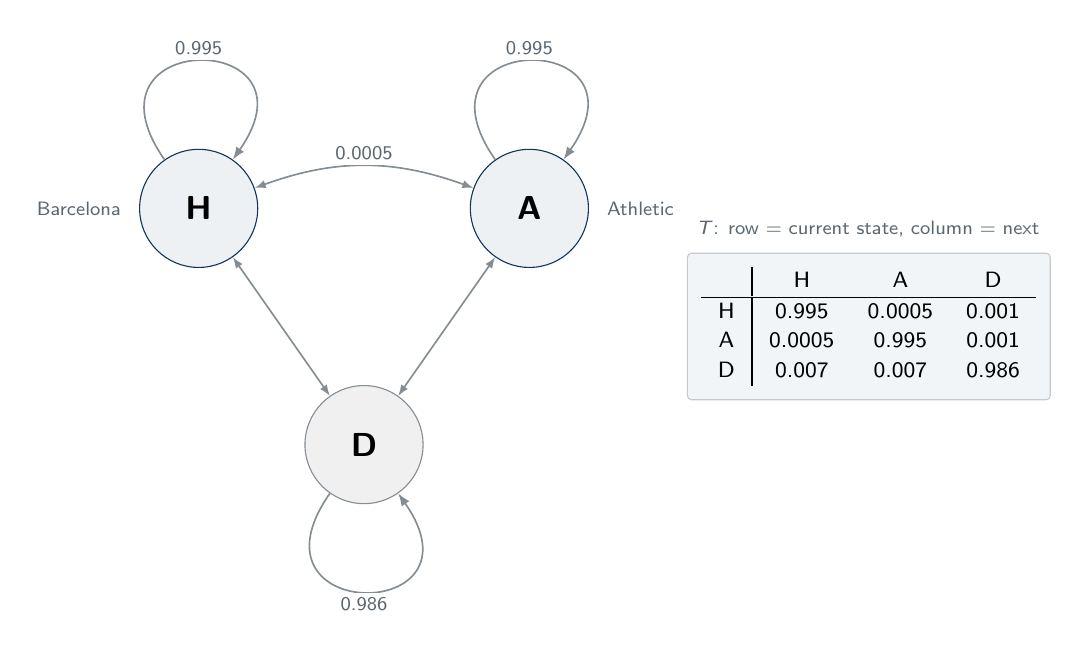
\begin{tikzpicture}[
  font=\scriptsize,
  state/.style={circle, draw=navy, fill=navy!7, minimum size=15mm, inner sep=0pt, font=\large\bfseries},
  dstate/.style={circle, draw=slate!75, fill=gray!12, minimum size=15mm, inner sep=0pt, font=\large\bfseries},
  edge/.style={-{Latex[length=1.6mm]}, draw=slate!75, line width=0.6pt},
  bi/.style={draw=slate!75, line width=0.6pt, {Latex[length=1.4mm]}-{Latex[length=1.4mm]}},
  lbl/.style={font=\scriptsize, text=slate, inner sep=2pt, fill=white}
]
\node[state] (H) at (0,0) {H};
\node[state] (A) at (4.2,0) {A};
\node[dstate] (D) at (2.1,-3.0) {D};
\node[font=\scriptsize, text=slate, left=3pt of H] {Barcelona};
\node[font=\scriptsize, text=slate, right=3pt of A] {Athletic};
% self loops
\draw[edge] (H) to[out=125,in=55,looseness=6] node[lbl,above]{$0.995$} (H);
\draw[edge] (A) to[out=125,in=55,looseness=6] node[lbl,above]{$0.995$} (A);
\draw[edge] (D) to[out=235,in=305,looseness=6] node[lbl,below]{$0.986$} (D);
% cross edges (numeric values in the matrix panel)
\draw[bi] (H) to[bend left=20] node[lbl,above]{$0.0005$} (A);
\draw[bi] (H) -- (D);
\draw[bi] (A) -- (D);
% transition matrix
\node[draw=slate!35, fill=mist, rounded corners=1.5pt, inner sep=5pt, anchor=west, font=\footnotesize] (mat) at (6.2,-1.5) {%
  \begin{tabular}{c|ccc}
   & H & A & D\\ \hline
  H & $0.995$ & $0.0005$ & $0.001$\\
  A & $0.0005$ & $0.995$ & $0.001$\\
  D & $0.007$ & $0.007$ & $0.986$
  \end{tabular}};
\node[font=\scriptsize, text=slate, anchor=south west] at ([yshift=2pt]mat.north west)
  {$T$: row = current state, column = next};
\end{tikzpicture}
\caption{The base HMM. The matrix $T$ (rows: current state; columns: next) and the self-loops
govern persistence. The geometric emission uses $\sigma=4.0$ m and $d_{dead}=8.0$ m; the
decode is a per-half Viterbi with 500 frames of context. Persistence ($p_{stay}=0.995$)
avoids fragmentation; leaving D is a little easier ($p_{dh}=0.007$) because confirmed saves
are already guaranteed by the events layer.}
\label{fig:hmm}
\end{figure}
\subsection{Perception: a second look, with a physical brake}

The ATD does not observe the ball in 43.1\,\% of the match (2.2\,\% estimated and 40.8\,\%
without estimate). Perception does not replace the ATD: it produces a \emph{second}
observation from the video for the frames where tactical tracking is not enough. The two
detectors are YOLO26x at 1024 px, trained on SoccerNet v3 H250 (CC-BY-4.0), the public
infactory-ai dataset (CC-BY-NC-4.0) and the martinjolif one (CC-BY-4.0) for the ball, and
SoccerNet/SN-Tracking-2023, martinjolif (players, CC-BY-4.0), keremberke (CC-BY-4.0) and manot
(MIT) for players; the full names are in \texttt{REPRODUCING.md}. No frame of this match and
no possession label entered the training.

The gate is kinematic, not a query to the truth: the ball cannot travel more than
$40\ \mathrm{m/s}\cdot\Delta t + 1\ \mathrm{m}$ between two accepted observations. A
detection outside that radius is discarded even if the detector is very confident; a
velocity prediction does not widen the gate, because the candidate must be reachable from
the last accepted point, not just from the predicted position. Re-acquisition requires two
mutually reachable detections. The own tracker anchors to the ATD and, in a gap, only
accepts measurements inside the gate; if it has neither anchor nor measurement, it does not
invent a position.

\subsection{Fusion: eight voters and an anchor}

Table~\ref{tab:weights} summarises the poll. Each source emits a distribution over H/A/D and
the effective weight is further reduced by its quality (ball confidence, player coverage,
sample age, whether the ATD already sees the ball). The HMM is the anchor; the other sources
have to win the disagreement, not replace it by decree.

\begin{table}[t]
\centering
\small
\caption{Poll voters and base weights. The weights are a design prior; they were not tuned
against the public ground truth. The HMM contributes 1.00 and each piece of evidence is added
as a likelihood update in the logit.}
\label{tab:weights}
\begin{tabular}{llr}
\toprule
Source & Role & Weight \\
\midrule
HMM ATD & anchor / temporal prior & 1.00 \\
YOLO ball & independent evidence & 0.10 \\
YOLO players & independent evidence & 0.10 \\
ATD ball & diagnostic (already in the emission) & 0.02 \\
ATD shape & diagnostic & 0.01 \\
Smart tags & diagnostic & 0.01 \\
Whistle & diagnostic & 0.02 \\
Events & hard $D$ (goals, saves) & 1.00 \\
\bottomrule
\end{tabular}
\end{table}

\subsection{Transitions: from smoothing to the event}

A kick is detected when the ball gains at least 6 m/s and leaves at 8--32 m/s towards a
player who is less than 2 m away; a control \emph{onset} is detected when a ball going at 7
m/s or more dies to 4 m/s or less next to a player who had been chasing it. Both are
attributed to the team of the nearest player, with per-team non-maximum suppression. The
pixel layer adds contacts inside the player box, clearance kicks and keeper hands; the area
geometry adds the keeper's catch when the ball dies inside his area.

An event only becomes a transition if all the conditions hold: the attributed team is
different from the current possessor; the ball is live (no ATD gap and no dead-ball window);
the attributed team was on the ball for at least 8 of the previous 15 frames; the
independent evidence favours the attributed team over the current one with a mean margin of
at least 0.10 during the next 2 s; and the ball stays live in the window. Then a decaying
logit pulse is applied to the incoming team, the transition matrix is relaxed around the
event and the spell is protected so the flicker merge does not absorb it.

\begin{figure}[t]
\centering
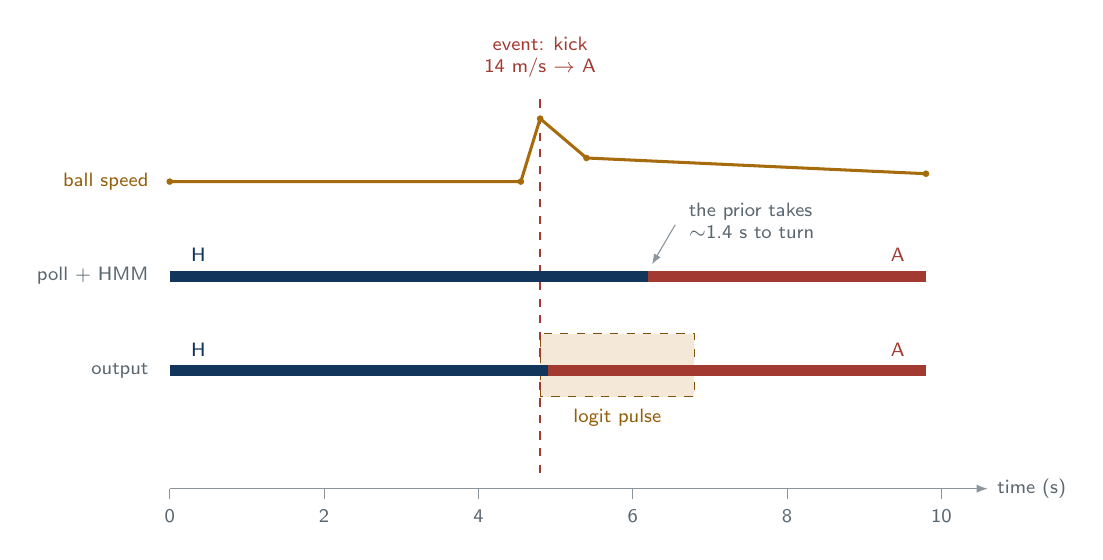
\begin{tikzpicture}[font=\scriptsize, x=0.98cm, y=1cm]
% pulse shading (behind the bands)
\fill[amber!16] (4.8,0.62) rectangle (6.8,1.42);
\draw[amber!70!black, dashed] (4.8,0.62) rectangle (6.8,1.42);
% time axis
\draw[-{Latex[length=1.4mm]}, slate!70] (0,-0.55) -- (10.6,-0.55) node[right, text=slate]{time (s)};
\foreach \t in {0,2,4,6,8,10} {
  \draw[slate!70] (\t,-0.55) -- (\t,-0.68);
  \node[text=slate, anchor=north] at (\t,-0.7) {\t};
}
% event line
\draw[dashed, crimson, line width=0.8pt] (4.8,-0.35) -- (4.8,4.5);
\node[crimson, anchor=south, align=center] at (4.8,4.55) {event: kick\\14 m/s $\to$ A};
% ball speed
\draw[line width=1.1pt, amber!90!black] (0,3.35) -- (4.55,3.35) -- (4.8,4.15) -- (5.4,3.65) -- (9.8,3.45);
\foreach \p in {(0,3.35),(4.55,3.35),(4.8,4.15),(5.4,3.65),(9.8,3.45)} \fill[amber!90!black] \p circle (1.2pt);
\node[anchor=east, text=amber!80!black] at (-0.15,3.35) {ball speed};
% poll band
\draw[line width=4pt, navy] (0,2.15) -- (6.2,2.15);
\draw[line width=4pt, crimson] (6.2,2.15) -- (9.8,2.15);
\node[navy, anchor=west] at (0.15,2.42) {H};
\node[crimson, anchor=east] at (9.65,2.42) {A};
\node[anchor=east, text=slate] at (-0.15,2.15) {poll + HMM};
% final band
\draw[line width=4pt, navy] (0,0.95) -- (4.9,0.95);
\draw[line width=4pt, crimson] (4.9,0.95) -- (9.8,0.95);
\node[navy, anchor=west] at (0.15,1.22) {H};
\node[crimson, anchor=east] at (9.65,1.22) {A};
\node[anchor=east, text=slate] at (-0.15,0.95) {output};
% annotations
\draw[-{Latex[length=1.3mm]}, slate!70] (6.55,2.8) -- (6.25,2.3);
\node[anchor=west, align=left, text=slate] at (6.6,2.85) {the prior takes\\$\sim$1.4 s to turn};
\node[text=amber!80!black, anchor=north] at (5.8,0.58) {logit pulse};
\end{tikzpicture}
\caption{Conceptual anatomy of a transition. The event (red line) is immediate; the poll with
HMM inertia takes time to turn; the pulse and the matrix relaxation move the boundary to the
event and protect the spell. The y-axis does not represent a physical magnitude: it is a
sketch, not a measured trace.}
\label{fig:transition}
\end{figure}

Besides the re-decode, the layer applies domain rules after the Viterbi: recovery of a ball
that went out and waits for the throw; restart after a false save; a possession that survives
a high ball that leaves and comes back; keeper's hand; long goal kick; and free-kick restart
after an offside call. These rules are documented in Section~\ref{sec:reglas}.
Table~\ref{tab:confusion} shows the confusion matrix of the public window.

\begin{table}[t]
\centering
\small
\caption{Confusion matrix of the public window (rows: GT; columns: prediction). The scored
total is 7,500; there are no abstentions in scored frames.}
\label{tab:confusion}
\begin{tabular}{lrrrr}
\toprule
GT $\backslash$ pred & H & A & D & total \\
\midrule
H & \textbf{3,369} & 80 & 5 & 3,454 \\
A & 31 & \textbf{2,526} & 20 & 2,577 \\
D & 26 & 71 & \textbf{1,372} & 1,469 \\
\bottomrule
\end{tabular}
\end{table}
% ----------------------------------------------------------------------------- reglas
\section{Possession rules}
\label{sec:reglas}

Table~\ref{tab:rules} fixes the boundary we have implemented. The common idea is that
possession is \emph{sticky}: the current team keeps it until there is enough evidence of a
change, not until a distance is minimal in one frame.

\begin{table}[t]
\centering
\footnotesize
\caption{Decision rules. ``Possession'' means H or A; ``D'' is a dead ball or out of play;
``X'' is abstention and only appears outside the scored halves.}
\label{tab:rules}
\begin{tabularx}{\textwidth}{@{}>{\raggedright\arraybackslash}p{4.1cm}X@{}}
\toprule
Situation & Decision \\
\midrule
Controlled ball & Team of the player closest to the ball; the emission weighs the distance
with a 4 m gaussian. If there is no clear margin, the previous possession is kept. \\
Duel or 50--50 & No change by geometry: an attributed event is needed and the independent
evidence must back the new team (margin $\geq 0.10$ for 2 s). \\
Loose or in-flight ball & More than 7 m from all players, the emission is uniform and the
prior decides. If it is moving at less than 2 m/s and the last touch is less than 5 s old,
the last toucher receives 70\,\% of the mass. \\
Ball parked on the line & Less than 2.5 m from a line, less than 1 m/s, the team at less than
1.35 m/s for 0.8 s (tolerating a 30\,\% flicker): the signature of a throw-in, corner or goal
kick; labelled D. \\
Observed offside & Ball observed beyond the line for at least 0.5 s: D. If the ball
disappears after crossing, at least 1 s: D. \\
Throw-in & The throwing team keeps the ball during the carry and the flight until the
opponent controls it for 3 consecutive frames, capped at 60 frames. If the ball moves with
nobody on it, it is not considered a restart. \\
Goal kick or long keeper & The team defending its goal receives the possession from the kick
and keeps it during the flight until a player receives it, contests it or it goes out. \\
Corner, free kick and offside & D until the ball is struck. In offside, the possession is not
assigned until the free kick is taken, not while the ball is placed. \\
Keeper with the ball & It is his team's possession, not D. A catch or clearance the camera
loses is stitched for up to 10 s if the keeper releases it to his team. \\
Goal or arbitral save & Hard D from the event to the restart. Two goals and 68 saves were
confirmed in the full match. \\
High ball that leaves and returns & If it returns to the same zone in a short window, with no
throw-in and no whistle, the same team's possession is stitched: the ball never really went
out. \\
Sub-1 s flicker & Absorbed into the previous label if it returns to it; X is never modified.
\\
\bottomrule
\end{tabularx}
\end{table}

Two decisions deserve explanation. The first is the \textbf{throw-in}: the tags do not carry
a team, so the team is attributed geometrically to the player who is on the ball; if nobody
is on the ball, there is no restart and we wait. The second is the \textbf{keeper}: a hand
inside his area is not a dead ball, it is his team's possession; the long throw from that
hand assigns the possession to the team defending that goal while the ball flies.
% ----------------------------------------------------------------------------- activos
\section{Assets used and discarded}

\paragraph{Used.}
\begin{itemize}
\item \textbf{Tactical ATD} (ball + 46 slots): distances, velocity, team shape, gaps and
last touch. It is the backbone of the HMM.
\item \textbf{Smart tags} (638 intervals, 14 codes): restart context, goals and saves; weak
vote, never a direct label. Throw-ins arrive without a team.
\item \textbf{Homography}: geometry validation (100\,\% of frames valid, median reprojection
error 0.24 px, p99 4.81 px) and viewer projection; not a label source.
\item \textbf{MP4 audio}: 274 whistle candidates; confirmed with low team movement and an
uncontrolled ball. Used in the events layer, not as an emission weight.
\item \textbf{Tactical video}: YOLO26x perception; 4,497 observations accepted in the public
window after the physical gate. It is the independent evidence of the poll.
\item \textbf{Two YOLO26x weights} (ball and players): trained only on external data;
published in the \texttt{champion-run} release with their checksums.
\item \textbf{Five minutes of public ground truth}: used to evaluate, tune the HMM
parameters and the bootstrap; never enters as an online input or in the detector training.
\end{itemize}

\paragraph{Discarded.}
\begin{itemize}
\item \textbf{MOSSE + GrayDiff + NanoTrack ensemble}: noisier than the ATD and unsynchronised
with the tactical tracking; abandoned.
\item \textbf{Broadcast video}: does not bring better geometry and is not needed for the
decision.
\item \textbf{Viewer Kalman layer}: never fed the model; removed so as not to keep a second
truth.
\item \textbf{Generic COCO weights}: side experiment excluded from the chain; the dedicated
detectors have better precision and recall on the ball.
\item \textbf{Tracker blend in the emission} (\code{est\_blend}): improved some frames but
created false changes in long gaps; the HMM keeps short gaps uniform.
\item \textbf{Flight rule} (\code{flight\_R}): the loose-ball + last-touch combination was
more stable; left disabled.
\item \textbf{Strong last touch} ($w_{lt}=0.2$): raised the spellF1 by about 0.005 but
lowered the macroF1 by about 0.019 and created a false H spell after a defensive touch at
frame 15,656.
\item \textbf{Two-state model} (live/dead + H/A): 0.547 spellF1 and 0.686 macroF1; worse than
the three-state HMM.
\item \textbf{Team vote by smart tags, walk/run fraction and gating by ball velocity}: each
one lowered the spellF1 between 0.03 and 0.07; discarded.
\item \textbf{Whistle as an emission}: duplicated evidence; only used to confirm saves in the
events layer.
\item \textbf{Identity by shirt colour}: not reliable at this resolution with these slots;
the team is taken from the nearest ATD slot and no identity is asserted.
\item \textbf{Manual labels or private ground truth}: forbidden by the rules; not used in any
step.
\end{itemize}

% ----------------------------------------------------------------------------- limitaciones
\section{Limitations}

\begin{itemize}
\item \textbf{The public window is small.} 17 possessions give a bootstrap interval of
[0.857; 0.971]; the parameters were tuned in that window and the full match is a
generalisation test, not a validation set. There is no cross-match validation.
\item \textbf{The penalty at frame 73,935 is missed.} The ATD stops seeing the ball for 55 s
around the kick; the last point before the gap is 13.5 m from the line, outside the 12 m
margin of the fallback, and the first re-observation is already behind the line and off the
posts. Loosening the rule would also accept the false goal at 57,283; precision was chosen
over recall and the failure is documented.
\item \textbf{Throw-in boundary at frame 164,968.} The release was detected in the thrower's
carry, not at the real kick (164,993); the 60-frame cap ends at 165,028, before the
reception (approximately 165,036). It is outside the public window, but it is an example of
the event-based boundary approximation.
\item \textbf{Full match: 259 H/A possessions}, mean 14.8 s and median 8.7 s over 158,857
scored frames. The mean approaches the 14.2 s of the public GT, but the median is shorter:
short episodes remain and there is some fragmentation in duels.
\item \textbf{ATD coverage.} Ball visible in 56.9\,\% of the frames; 2.2\,\% estimated and
40.8\,\% without estimate. The 46 slots are not a guaranteed 11v11: there are frames with
more than 11 tracks per team (maximum 35 visible slots), probably substitutes, staff or
duplicates. No identity is inferred.
\item \textbf{Smart tags.} They cover 70.1\,\% of the match; their team vote is weak and
throw-ins do not carry a team. The transition layer does not depend on them for the main
decision.
\item \textbf{Perception.} The YOLO inference is deterministic with the same weights,
resolution and library versions, but small GPU differences can change the cache. The cache
is not published because it is match-derived tracking; its local SHA-256 is documented as a
reference. If it does not match, the reproducibility of the CSV is not guaranteed.
\item \textbf{Precision over recall.} The events layer is designed not to invent
transitions: it may miss deflections or possessions of less than a second. The result is 18
predicted possessions against 17 real ones in the public window.
\end{itemize}

% ----------------------------------------------------------------------------- reproduccion
\section{Reproduction}

The public repository is
\href{https://github.com/BinarySandia04/Xplainable-soccer-predictor}{github.com/BinarySandia04/Xplainable-soccer-predictor}.
The match data is not distributed with the code; it is obtained from the organisers' bundle.
The two weights are published in the release
\href{https://github.com/BinarySandia04/Xplainable-soccer-predictor/releases/tag/champion-run}{\texttt{champion-run}};
the final CSV is in \texttt{deliverables/}. The perception cache is not published: it is
match-derived tracking.

\begin{lstlisting}
python -m venv .venv
.venv/bin/pip install -r requirements.txt

# 1. Perception (GPU, once). The weights are downloaded from the champion-run release.
.venv/bin/python farm_perceive.py --video data/tactical/BAR-ATH_tactical-001.mp4 \
    --ball-weights ball_yolo26x_1024_clu.pt \
    --players-weights players_yolo26x_1024_clu.pt \
    --output-dir possession_lab/outputs

# 2. Multi-source fusion (deterministic CPU).
.venv/bin/python -m possession_lab fusion \
    --perception possession_lab/outputs/perception_new_fixed.npz

# 3. Transition layer: generates the submitted CSV.
.venv/bin/python -m possession_lab transitions \
    --perception possession_lab/outputs/perception_new_fixed.npz \
    --fusion possession_lab/outputs/fusion.npz

# 4. Official validation of the exact file that is uploaded.
cp possession_lab/outputs/transition_predictions.csv Xplainable.csv
.venv/bin/python evaluation/validate_submission.py Xplainable.csv

# 5. Tests (375 passed, 4 subtests).
PYTHONPATH=. .venv/bin/python -m pytest possession_lab/tests/ -q
\end{lstlisting}

\begin{samepage}
If your local perception cache matches the reference checksums, steps 2 and 3 are pure CPU
and reproduce the CSV byte for byte. The expected verification sums are (the first two rows
are local caches, not published):

\begin{center}
\footnotesize
\begin{tabularx}{\textwidth}{@{}>{\raggedright\arraybackslash}p{4.6cm}@{\hspace{8pt}}X@{}}
\toprule
Artefact & SHA-256 \\
\midrule
\code{perception\_new\_fixed.npz} & \sha{9dddaa128dc9eb39eae8419958e4252bb5ed65a423418f33a08ac835ff855f1b} \\
\code{fusion.npz} & \sha{e7ea998b74b963af25413d1938bf5659e56efec1f155e0a668c4dbf4dcae0369} \\
\code{Xplainable.csv} & \sha{9d79ad4bd83327f03299e02919623ef89215145eecabf1aa0a1a9bb4a5ce66fb} \\
\bottomrule
\end{tabularx}
\end{center}
\end{samepage}

The CSV has 199,319 data rows, frames 0--199,318 in order, labels in $\{H,A,D,X\}$, no empty
cells and no index column. The official validator returns \texttt{OK} and the public metrics
match Table~\ref{tab:metrics}. The perception was run once; everything afterwards is
deterministic CPU. The local viewer (\code{.venv/bin/python -m possession\_lab viewer} with
the three artefacts) allows synchronising the video, the label, the ball and the reasons of
each change.

% ----------------------------------------------------------------------------- cierre
\section{Conclusion}

The main contribution is not a bigger detector, but separating two problems that are usually
mixed: \emph{stabilising} possession and \emph{changing} possession at the right moment. The
HMM solves the first with a strong prior and an explicit gap model; the transition layer
solves the second with physical events, team attribution and independent evidence. The YOLO
perception and the poll add a second look without letting a noisy detection replace the
validated model. The result is an auditable system, reproducible on CPU, with a documented
failure instead of a hidden number: 0.9257 public spellF1, 0.9661 macroF1 and 18 predicted
possessions against 17 real ones.

\subsection*{Compliance and delivery}

\begin{center}
\footnotesize
\begin{tabularx}{\textwidth}{@{}>{\raggedright\arraybackslash}p{3.9cm}X@{}}
\toprule
Requirement & Evidence \\
\midrule
Algorithmic labels & The 199,319 labels come out of the
\texttt{fusion} $\to$ \texttt{transitions} chain; there is no painting, manual correction or
heuristic applied by hand to the CSV. \\
No private ground truth & The only truth used is the 7,500-frame public CSV; it was used to
evaluate, tune parameters and the bootstrap, never as an online input or for manual
labelling. \\
Reproducible & The repository includes pinned dependencies, the weights in the release,
commands and SHA-256 sums. The submitted CSV matches \texttt{transition\_predictions.csv}
byte for byte. \\
Data not redistributed & \texttt{data/} is excluded from Git; no video, tracking or crops
are published. Only code, weights trained on external data and the solution labels are
published. \\
Format & Header \texttt{frame,label}, 199,319 data rows, frames 0--199,318 in order, labels
in $\{H,A,D,X\}$, UTF-8, no index. Official validator: \texttt{OK}. \\
Delivery & Team \textbf{Xplainable}: \texttt{Xplainable.csv} and \texttt{Xplainable.pdf};
public repository and a single response in the form. \\
\bottomrule
\end{tabularx}
\end{center}

\paragraph{Where to look.}
The repository is organised by stages so each decision can be audited separately.

\begin{center}
\footnotesize
\begin{tabularx}{\textwidth}{@{}>{\raggedright\arraybackslash}p{6.1cm}X@{}}
\toprule
File & Content \\
\midrule
\code{possession\_lab/model.py} & Emissions, Viterbi, forward--backward and transition matrix. \\
\code{possession\_lab/features.py} & Geometry, gaps, last touch, movement and dead-ball signals. \\
\code{possession\_lab/fusion/voters.py} & The eight voters, their roles and the poll weights. \\
\code{possession\_lab/fusion/transitions.py} & Event detection, gates, re-decode and restart rules. \\
\code{possession\_lab/events.py} & Goals, saves and $D$ overrides. \\
\code{possession\_lab/explain.py} & Ordered reasons of each possession change. \\
\code{evaluation/validate\_submission.py} & Official validator of the format. \\
\code{REPRODUCING.md} & Full chain, dependencies, checksums and limits. \\
\bottomrule
\end{tabularx}
\end{center}

\vspace{2pt}
{\footnotesize\color{slate}Document generated from the artefacts of the
\texttt{champion-run} release. The figures of Table~\ref{tab:metrics} and the verification
sums can be reproduced with the commands of Section~7.}

\end{document}
